Die Prototypen bestehen im Frontend aus React und wurden mit Create React App erstellt. Create React App ist ein Command Line Tool (CLI), das ein Projekt mit dem gewünschten Namen erstellt, eine initiale Projektstruktur generiert (vgl. \autoref{fig:init}) und die dafür benötigten Abhängigkeiten installiert~\cite{create-react}.
\begin{figure}[H]
  \centering
  \begin{subfigure}[t]{0.4\textwidth}
          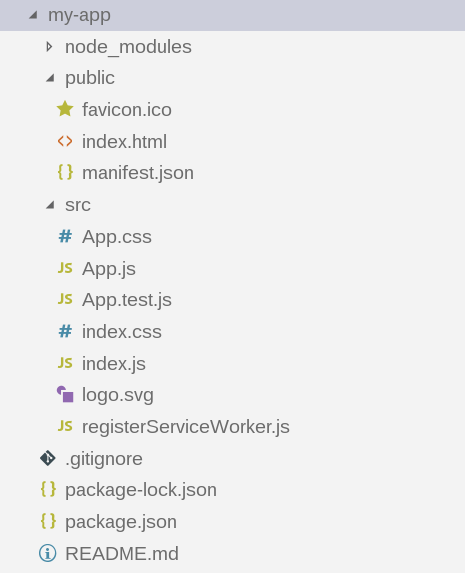
\includegraphics[width=\textwidth]{Ordnerstruktur}
          \caption{Die initiale Projektstruktur}
          \label{fig:init}
  \end{subfigure}
  ~
  \begin{subfigure}[t]{0.4\textwidth}
          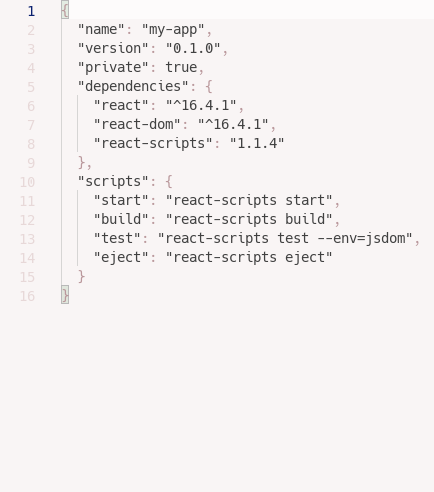
\includegraphics[width=\textwidth]{rca-package}
          \caption{Die initiale package.json Datei}
          \label{fig:init2}
  \end{subfigure}
  \grayRule
  \caption[Create React App: initiale Testapplikation]{einer mit Create React App erstellten Testapplikation}
  \label{fig:create-react-app}
\end{figure}
%
Diese sind im Verzeichnis node\_modules installiert.
Außerdem ist ein Service Worker enthalten, der die \gls{Assets} cacht.
Als Template gibt es nun die \tt{public/index.html}-- Datei. In der \tt{index.js}--Datei werden die React--Komponenten und der Service Worker initialisiert.
Alle \tt{App.*}--Dateien umfassen eine minimale Beispielanwendung.
In der generierten \tt{package.json}--Datei (vgl. \autoref{fig:init2}), befinden sich Informationen über die Anwendung und ihre Abhängigkeiten.
Im Unterpunkt \tt{scripts} werden Kommandozeilen-Aufrufe definiert und können mit dem Befehl \tt{npm run} aufgerufen werden.